% !TeX root = ../main.tex

% Edit this title for each week's entry.
\section{Week 6: Variance Decomposition Part 1}

\heading{Module Outline}
\begin{itemize}
    \item Decomposition of the sum of squares
    \item ANOVA test for overall significance
    \item Partial $F$ test
\end{itemize}
Today we think about the \textbf{marginal} variance of $Y$, $\Var(Y)$, in addition to
the \textbf{conditional} variance of $Y\mid X$, $\Var(Y\mid X)$.

\subsection{Variation in Linear Regression}

\begin{remark}[Variation and Strength of a Linear Relationship]
    \begin{itemize}
        \item So far we treat the predictors $X$ as fixed and fit the model that minimizes the
        RSS (variation around the line of best fit).
        \item Variation tells us how strong the linear relationship is: \textbf{less noise
        around the trend} $\to$ stronger linear relationship $\to$ the predictor(s) explain
        the spread of $Y$ better.
        \item The $t$-test for $\beta_j$ also uses this variation around the line to decide
        whether there is a significant linear relationship between $X_j$ and $Y$ in the
        presence of the other predictors.
    \end{itemize}
\end{remark}

\begin{center}
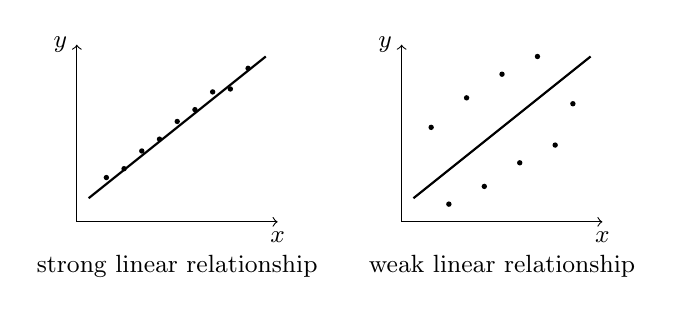
\begin{tikzpicture}[scale=0.75]
    \begin{scope}
        \draw[->] (0,0) -- (3.4,0) node[below]{\small $x$};
        \draw[->] (0,0) -- (0,3) node[left]{\small $y$};
        \draw[thick] (0.2,0.4) -- (3.2,2.8);
        \foreach \p in {(0.5,0.75),(0.8,0.9),(1.1,1.2),(1.4,1.4),(1.7,1.7),(2.0,1.9),(2.3,2.2),(2.6,2.25),(2.9,2.6)}
            \fill \p circle (1.3pt);
        \node[below] at (1.7,-0.4) {\small strong linear relationship};
    \end{scope}
    \begin{scope}[xshift=5.5cm]
        \draw[->] (0,0) -- (3.4,0) node[below]{\small $x$};
        \draw[->] (0,0) -- (0,3) node[left]{\small $y$};
        \draw[thick] (0.2,0.4) -- (3.2,2.8);
        \foreach \p in {(0.5,1.6),(0.8,0.3),(1.1,2.1),(1.4,0.6),(1.7,2.5),(2.0,1.0),(2.3,2.8),(2.6,1.3),(2.9,2.0)}
            \fill \p circle (1.3pt);
        \node[below] at (1.7,-0.4) {\small weak linear relationship};
    \end{scope}
\end{tikzpicture}
\end{center}

\begin{remark}[Variation in SLR and $t$-Tests]
    In SLR, $y_i=\beta_0+\beta_1x_i+\varepsilon_i$.
    \begin{itemize}
        \item If $\beta_1=0$, then $y_i=\beta_0+\varepsilon_i$ and $\hat\beta_0=\bar y$: variation
        around a \textbf{horizontal line}. \aside{$H_0:\beta_1=0$ is the model $\hat y_i=\bar y$.}
        \item When there is a linear relationship, generally $\hat y_i\neq\bar y$.
        \item Testing $H_0:\beta_1=0$ compares $\hat\beta_1-0$ to the variation in estimating
        $\hat\beta_1$: $\Var(\hat\beta_1)=\frac{\sigma^2}{\sum(x_i-\bar x)^2}$ is estimated by
        $\frac{s^2}{\sum(x_i-\bar x)^2}$, which includes $s^2=\frac{\sum(y_i-\hat y_i)^2}{n-2}$.
        \item For the $t$-test to indicate a significant linear relationship, the
        \rb{$\hat y_i-\bar y$} (fitted line vs.\ horizontal line) across all observations would
        need to overall be larger than the residual differences \rb{$y_i-\hat y_i$}.
    \end{itemize}
\end{remark}

\subsection{Sum of Squares Decomposition}

\begin{theorem}[Law of Total Variance (STA237/220)]
    \[\boxed{V[Y]=\underbrace{E\big[V[Y\mid X]\big]}_{\text{unexplained}}+\underbrace{V\big[E[Y\mid X]\big]}_{\text{explained}}}\]
    If $X$ is discrete, the variance of $Y$ is the sum of the \textbf{within-group}
    (unexplained) variance and the \textbf{between-group} (explained by group membership)
    variance. In regression: the total variability of $Y$ is the variance that cannot be
    explained by $X$ plus the variance that can be explained by $X$.
    \aside{Don't worry if you don't remember this.}
\end{theorem}

\begin{definition}[Total Sum of Squares]
    We are interested in explaining $\Var(Y)$ \aside{(not conditional on $X$)}: the total
    amount of variation in $Y$, quantified by
    \[SST=SS_{yy}=\sum(y_i-\bar y)^2,\]
    the numerator of $\widehat{\Var}(Y)$.
    \begin{itemize}
        \item Each predictor added to the model explains a little bit of this variation; how
        much depends on the slope $\hat\beta_j$.
        \item There is always some variation left over: the random error term can never be modelled.
    \end{itemize}
    Each deviation splits as
    \[y_i-\bar y=\underbrace{(y_i-\hat y_i)}_{\text{residual}}+\underbrace{(\hat y_i-\bar y)}_{\text{fitted vs.\ mean}}\]
\end{definition}

\begin{center}
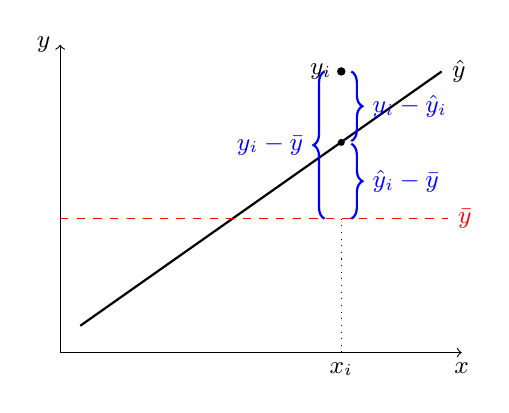
\begin{tikzpicture}[scale=0.85]
    \draw[->] (0,0) -- (6,0) node[below]{\small $x$};
    \draw[->] (0,0) -- (0,4.6) node[left]{\small $y$};
    \draw[thick] (0.3,0.4) -- (5.7,4.2) node[right]{\small $\hat y$};
    \draw[red,dashed] (0,2) -- (5.8,2) node[right]{\small $\bar y$};
    \fill (4.2,4.2) circle (1.8pt) node[left]{\small $y_i$};
    \fill (4.2,3.14) circle (1.5pt);
    \draw[blue,thick,decorate,decoration={brace,amplitude=4pt}] (4.35,4.2) -- (4.35,3.16) node[midway,right=4pt]{\small $y_i-\hat y_i$};
    \draw[blue,thick,decorate,decoration={brace,amplitude=4pt}] (4.35,3.12) -- (4.35,2.0) node[midway,right=4pt]{\small $\hat y_i-\bar y$};
    \draw[blue,thick,decorate,decoration={brace,amplitude=4pt,mirror}] (3.95,4.2) -- (3.95,2.0) node[midway,left=4pt]{\small $y_i-\bar y$};
    \draw[dotted] (4.2,0) node[below]{\small $x_i$} -- (4.2,2);
\end{tikzpicture}
\\[2pt] \textit{\small Graphical depiction of $y_i-\bar y=(y_i-\hat y_i)+(\hat y_i-\bar y)$ (after Sheather, p.\ 29).}
\end{center}

\begin{definition}[The Three Sums of Squares]
    \begin{itemize}
        \item \rb{Total} variation in $Y$ prior to fitting a model (ignoring predictors):
        \[SST=\sum(y_i-\bar y)^2\ \propto\ \Var(Y)\]
        \item \rb{Explained} variation, by the predictors/the model:
        \[SS_{reg}=\sum(\hat y_i-\bar y)^2\ \propto\ V\big(E(Y\mid X)\big)\]
        \item \rb{Unexplained} variation left over after fitting the model:
        \[RSS=\sum(y_i-\hat y_i)^2=\sum\hat\epsilon_i^2\ \propto\ E\big(V(Y\mid X)\big)\]
    \end{itemize}
    \textbf{Sum of squares decomposition} (analogous to the law of total variance):
    \[\boxed{SST=SS_{reg}+RSS}\]
    \aside{Other sources may use different names and abbreviations for these.}
\end{definition}

\begin{definition}[Coefficient of Determination $R^2$]
    The proportion of the variation in the response that is predictable from/explained by
    the predictor(s):
    \[\boxed{R^2=1-\frac{RSS}{SST}=\frac{SS_{reg}}{SST}}\]
    In SLR, $R^2=\mathrm{corr}(X,Y)^2$.
\end{definition}

\begin{remark}[Interpreting $SS_{reg}$]
    \begin{itemize}
        \item $SS_{reg}$ is how much of the overall variation in $Y$ is explained by $X$. If $X$
        is categorical it is often called the \textbf{between-group} SS, and RSS the
        \textbf{within-group} SS.
        \item Sums of squares measure squared distance, like the numerator of a sample variance.
        \item If each $\hat y_i$ is generally \textbf{close} to $\bar y$, $SS_{reg}\approx0$: the
        model isn't doing much to explain $Y$.
        \item If each $\hat y_i$ is generally \textbf{far} from $\bar y$, $SS_{reg}$ is large: the
        predictors explain a lot of what happens with $Y$.
    \end{itemize}
\end{remark}

\begin{center}
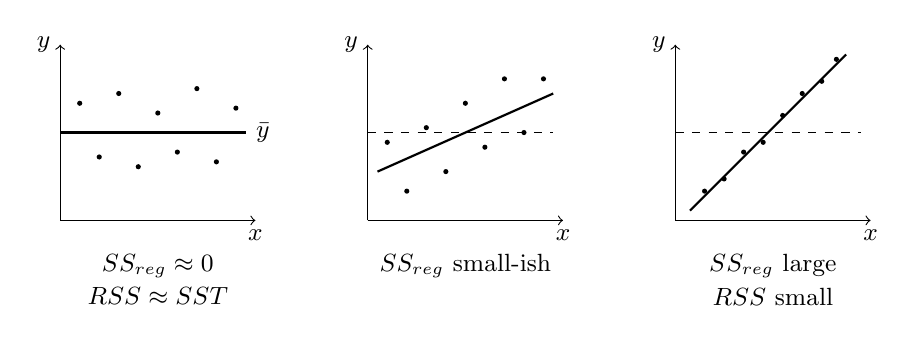
\begin{tikzpicture}[scale=0.62]
    \begin{scope}
        \draw[->] (0,0) -- (4,0) node[below]{\small $x$};
        \draw[->] (0,0) -- (0,3.6) node[left]{\small $y$};
        \draw[thick] (0,1.8) -- (3.8,1.8) node[right]{\small $\bar y$};
        \foreach \p in {(0.4,2.4),(0.8,1.3),(1.2,2.6),(1.6,1.1),(2.0,2.2),(2.4,1.4),(2.8,2.7),(3.2,1.2),(3.6,2.3)}
            \fill \p circle (1.5pt);
        \node[align=center,below] at (2,-0.5) {\small $SS_{reg}\approx0$\\\small $RSS\approx SST$};
    \end{scope}
    \begin{scope}[xshift=6.3cm]
        \draw[->] (0,0) -- (4,0) node[below]{\small $x$};
        \draw[->] (0,0) -- (0,3.6) node[left]{\small $y$};
        \draw[dashed] (0,1.8) -- (3.8,1.8);
        \draw[thick] (0.2,1.0) -- (3.8,2.6);
        \foreach \p in {(0.4,1.6),(0.8,0.6),(1.2,1.9),(1.6,1.0),(2.0,2.4),(2.4,1.5),(2.8,2.9),(3.2,1.8),(3.6,2.9)}
            \fill \p circle (1.5pt);
        \node[align=center,below] at (2,-0.5) {\small $SS_{reg}$ small-ish};
    \end{scope}
    \begin{scope}[xshift=12.6cm]
        \draw[->] (0,0) -- (4,0) node[below]{\small $x$};
        \draw[->] (0,0) -- (0,3.6) node[left]{\small $y$};
        \draw[dashed] (0,1.8) -- (3.8,1.8);
        \draw[thick] (0.3,0.2) -- (3.5,3.4);
        \foreach \p in {(0.6,0.6),(1.0,0.85),(1.4,1.4),(1.8,1.6),(2.2,2.15),(2.6,2.6),(3.0,2.85),(3.3,3.3)}
            \fill \p circle (1.5pt);
        \node[align=center,below] at (2,-0.5) {\small $SS_{reg}$ large\\\small $RSS$ small};
    \end{scope}
\end{tikzpicture}
\end{center}

\begin{example}[Adding a Predictor]
    Data with a curved (decreasing, convex) trend:
    \begin{itemize}
        \item \texttt{y \textasciitilde{} x}: some points are far from the line of best fit, so
        RSS is somewhat large and $SS_{reg}$ somewhat large.
        \item \texttt{y \textasciitilde{} x + x\^{}2}, $\hat y=\hat\beta_0+\hat\beta_1x+\hat\beta_2x^2$:
        \dbb{RSS decreases, $SS_{reg}$ increases}, and \dbb{SST stays the same} (the data did not change).
    \end{itemize}
\end{example}

\begin{remark}[Picture: Conditional Distributions (Wikipedia ANOVA figures)]
    Picture the marginal distribution of $Y$ (spread $V(Y)$, centred at $E(Y)=\bar y$) next to
    the conditional distributions $Y\mid X=x_i$ (spreads $V(Y\mid X_i)$, centred at $E(Y\mid X=x_i)$).
    \begin{itemize}
        \item \textbf{No fit}: all $E(Y\mid X=x_i)$ sit at $\bar y$ $\Rightarrow$ RSS big, $SS_{reg}$
        small; $X$ does not explain how $Y$ changes.
        \item \textbf{OK fit}: the conditional means spread out $\Rightarrow$ $SS_{reg}$ bigger, RSS smaller.
        \item \textbf{Very good fit}: conditional means spread widely and each $V(Y\mid X_i)$ is
        narrow $\Rightarrow$ $SS_{reg}$ very large; $X$ explains a large part of the variance of $Y$.
    \end{itemize}
\end{remark}

\subsection{Proof of the Decomposition}

\begin{remark}[Strategy]
    Show $\sum(y_i-\bar y)^2=\sum(\hat y_i-\bar y)^2+\sum(y_i-\hat y_i)^2$ by expanding the
    squares and showing the cross terms are 0. \aside{Proofs of this type appear in many
    upper-year STA courses --- decomposing sums of squares is a VERY important skill.}
    \\ Recall from Module 1: \hly{\sum_{i=1}^n x_i\hat\varepsilon_i=0} and
    \hly{\sum_{i=1}^n\hat\varepsilon_i=0}. This holds for MLR too: the residuals are
    uncorrelated with every predictor and still sum to 0 (given an intercept). In matrix
    form, \hly{\hat{\boldsymbol\epsilon}'\mathbf{X}=\mathbf{0}}.
\end{remark}

\begin{proposition}[$\hat{\boldsymbol\epsilon}'\mathbf{X}=\mathbf{0}$]
    Using $\hat{\mathbf{Y}}=\mathbf{H}\mathbf{Y}$ and $\mathbf{H}'=\mathbf{H}$:
    \begin{align*}
        (\mathbf{Y}-\hat{\mathbf{Y}})'\mathbf{X}
        &=(\mathbf{Y}'-\hat{\mathbf{Y}}')\mathbf{X}=\big(\mathbf{Y}'-(\mathbf{H}\mathbf{Y})'\big)\mathbf{X}=(\mathbf{Y}'-\mathbf{Y}'\mathbf{H}')\mathbf{X}\\
        &=\mathbf{Y}'(\mathbf{I}-\mathbf{H})\mathbf{X}=\mathbf{Y}'\big(\mathbf{I}-\mathbf{X}(\mathbf{X}'\mathbf{X})^{-1}\mathbf{X}'\big)\mathbf{X}\\
        &=\mathbf{Y}'\big(\mathbf{X}-\mathbf{X}\underbrace{(\mathbf{X}'\mathbf{X})^{-1}\mathbf{X}'\mathbf{X}}_{\mathbf{I}}\big)=\mathbf{Y}'(\mathbf{X}-\mathbf{X})=\mathbf{0}
    \end{align*}
    So $\sum_{i=1}^n x_{ij}\hat\varepsilon_i=0$ for all $j$, and $\sum_{i=1}^n\hat\varepsilon_i=0$
    since the first column of the design matrix is $(1,\dots,1)'$.
\end{proposition}

\begin{proof}[Proof of $SST=SS_{reg}+RSS$ (scalars)]
    \[\sum(y_i-\bar y)^2=\sum\big((y_i-\hat y_i)+(\hat y_i-\bar y)\big)^2
    =\underbrace{\sum(y_i-\hat y_i)^2}_{RSS}+\underbrace{\sum(\hat y_i-\bar y)^2}_{SS_{reg}}+\underbrace{2\sum(y_i-\hat y_i)(\hat y_i-\bar y)}_{\text{show }=0}\]
    With $y_i-\hat y_i=\hat\varepsilon_i$ and $\bar y$ not changing with $i$:
    \[2\sum\hat\varepsilon_i(\hat y_i-\bar y)=2\Big(\sum\hat\varepsilon_i\hat y_i-\bar y\underbrace{\sum\hat\varepsilon_i}_{0}\Big)\]
    and
    \[\sum\hat\varepsilon_i\hat y_i=\sum\hat\varepsilon_i(\hat\beta_0+\hat\beta_1x_{i1}+\hat\beta_2x_{i2}+\cdots)
    =\hat\beta_0\underbrace{\sum\hat\varepsilon_i}_{0}+\hat\beta_1\underbrace{\sum\hat\varepsilon_ix_{i1}}_{0}+\hat\beta_2\underbrace{\sum\hat\varepsilon_ix_{i2}}_{0}+\cdots=0\]
    So the cross terms are 0 and $SST=SS_{reg}+RSS$.
\end{proof}

\begin{proof}[Proof of $SST=SS_{reg}+RSS$ (vectors/matrices)]
    Define $\|\mathbf{a}\|^2=\sum_{k=1}^\ell a_k^2=\mathbf{a}\cdot\mathbf{a}=\mathbf{a}'\mathbf{a}$
    and $\mathbb{1}=(1,\dots,1)'$. We want
    \[\underbrace{\|\mathbf{Y}-\bar y\mathbb{1}\|^2}_{SST}=\underbrace{\|\hat{\mathbf{Y}}-\bar y\mathbb{1}\|^2}_{SS_{reg}}+\underbrace{\|\hat{\boldsymbol\epsilon}\|^2}_{RSS}\]
    Expanding,
    \[\|(\mathbf{Y}-\hat{\mathbf{Y}})+(\hat{\mathbf{Y}}-\bar y\mathbb{1})\|^2=\|\mathbf{Y}-\hat{\mathbf{Y}}\|^2+\|\hat{\mathbf{Y}}-\bar y\mathbb{1}\|^2+\underbrace{2(\mathbf{Y}-\hat{\mathbf{Y}})'(\hat{\mathbf{Y}}-\bar y\mathbb{1})}_{\text{show }=0}\]
    and with $\mathbf{Y}-\hat{\mathbf{Y}}=\hat{\boldsymbol\epsilon}$, $\hat{\mathbf{Y}}=\mathbf{X}\hat{\boldsymbol\beta}$:
    \[2\hat{\boldsymbol\epsilon}'(\hat{\mathbf{Y}}-\bar y\mathbb{1})=2\underbrace{\hat{\boldsymbol\epsilon}'\mathbf{X}}_{\mathbf{0}}\hat{\boldsymbol\beta}-2\bar y\underbrace{\hat{\boldsymbol\epsilon}'\mathbb{1}}_{\sum\hat\varepsilon_i=0}=0\qedhere\]
\end{proof}

\begin{definition}[Degrees of Freedom]
    Each term has a degree of freedom (like the denominator of a sample variance):
    \begin{itemize}
        \item $SST$: $n-1$ \aside{(df when estimating $\mu$ with $\bar y$)}
        \item $RSS$: $n-p-1$, $p=$ number of predictors \aside{(df when fitting the regression model)}
        \item $SS_{reg}$: $(p+1)-1=p$ \aside{(we have $p+1$ $\beta_j$'s)}
    \end{itemize}
    DFs decompose too: \hly{n-1=(n-p-1)+p}.
\end{definition}

\subsection{ANOVA Test for Overall Significance}

\begin{remark}[Why We Need Another Test]
    \begin{itemize}
        \item The $t$-test on $\beta_j$ ($H_0:\beta_j=0$, $t^*=\hat\beta_j/SE(\hat\beta_j)$) in
        \textbf{SLR} is equivalent to testing whether a linear relationship exists in the model.
        \item In \textbf{MLR} it only says whether $X_j$ is linearly related to $Y$ \emph{in the
        presence of the others} --- not whether a linear relationship exists in the model in general.
    \end{itemize}
\end{remark}

\begin{example}[House Pricing (Simulated)]
    True model $Y=1+3X_1+2X_2+\epsilon$, $X_1=$ \#bedrooms, $X_2=$ \#bathrooms, with
    $X_1\approx X_2$ (very correlated):
\begin{verbatim}
n = 100
set.seed(1234)
numBedrooms  = sample(c(0,1,2,3,4,5), size = n, replace = TRUE)
numBathrooms = numBedrooms + round(runif(n,-0.51,0.51))  # differ by at most 1
sellPrice    = 1 + 3*numBedrooms + 2*numBathrooms + rnorm(n, 0, 3)
model <- lm(sellPrice ~ numBedrooms + numBathrooms)

             Estimate Std. Error t value Pr(>|t|)
(Intercept)    1.9156     0.5956   3.216  0.00177 **
numBedrooms    2.3661     2.2732   1.041  0.30053
numBathrooms   2.4111     2.2772   1.059  0.29232
Residual standard error: 3.182 on 97 degrees of freedom
Multiple R-squared: 0.879, Adjusted R-squared: 0.8765
F-statistic: 352.4 on 2 and 97 DF, p-value: < 2.2e-16
\end{verbatim}
    \db{Neither \#beds nor \#baths is significant in the presence of the other, but we
    \dbb{know} there is a linear relationship from the data-generating process.} Scatterplots
    of \texttt{sellPrice} vs.\ either predictor show a clear linear trend, and each SLR model
    agrees:
    \begin{center}
        \begin{tabular}{lrrrr}
            \toprule
            Model & $\hat\beta_1$ & SE & $t$ & p-value \\
            \midrule
            \texttt{sellPrice \textasciitilde{} numBedrooms} & 4.7654 & 0.1798 & 26.509 & $<2\times10^{-16}$ \\
            \texttt{sellPrice \textasciitilde{} numBathrooms} & 4.7740 & 0.1800 & 26.515 & $<2\times10^{-16}$ \\
            \bottomrule
        \end{tabular}
    \end{center}
    Unsurprising since $X_1\approx X_2$. How do we test, in the MLR model, whether at least one
    predictor explains enough of the variation in $Y$? \textbf{Use the sum of squares decomposition.}
\end{example}

\begin{remark}[Building a Test from the Decomposition]
    \begin{itemize}
        \item Significant linear relationship $=$ a significant amount of the variation in the
        response was explained by the model: $SS_{reg}$ large, explaining a large portion of $SST$.
        \item A good model has $SS_{reg}$ much larger than $RSS$; by the decomposition,
        $SS_{reg}/SST$ large necessarily means $RSS/SST$ small.
        \item The test of overall significance checks whether $SS_{reg}$ is statistically
        significantly bigger than $RSS$.
        \item Every dataset has a different $SST$, so we can't look at $SS_{reg}/SST$ directly.
    \end{itemize}
\end{remark}

\begin{definition}[ANOVA Test of Overall Significance]
    Split $\boldsymbol\beta=(\beta_0,\boldsymbol\beta_1)'$ and test
    \[H_0:\boldsymbol\beta_1=\mathbf{0}\ \ (\beta_1=\beta_2=\cdots=\beta_p=0)\quad\text{vs.}\quad H_A:\boldsymbol\beta_1\neq\mathbf{0}\ \ (\text{at least one slope}\neq0)\]
    Assuming $H_0$ is true,
    \[\boxed{F^*=\frac{SS_{reg}/p}{RSS/(n-p-1)}=\frac{MS_{reg}}{MSR}\sim F(p,\,n-p-1)}\]
    with $SS_{reg}=\sum(\hat y_i-\bar y)^2$, $RSS=\sum(y_i-\hat y_i)^2$.
    \aside{$F(df_1,df_2)$: numerator df, denominator df.} Dividing each SS by its df
    standardizes it, giving the \textbf{Mean Squares Regression} $MS_{reg}$ and the
    \textbf{Mean Squares Residual} $MSR$.
\end{definition}

\begin{center}
    \begin{tabular}{lcccc}
        \toprule
        Source & DF & Sum of Squares & Mean Squares & $F$ value \\
        \midrule
        Regression & $p$ & $SS_{reg}$ & $MS_{reg}=SS_{reg}/p$ & $MS_{reg}/MSR$ \\
        Residual & $n-p-1$ & $RSS$ & $MSR=RSS/(n-p-1)$ & -- \\
        Total & $n-1$ & $SST$ & -- & -- \\
        \bottomrule
    \end{tabular}
    \\[2pt] \textit{\small ANOVA table summarizing the test components.}
\end{center}

\begin{remark}[Aside: ANOVA for Group Means (STA288)]
    ANOVA tests group differences: $H_0:\mu_1=\mu_2=\cdots=\mu_k$ (same mean in all $k$
    categories) vs.\ $H_A$: at least one $\mu_j$ differs, using the same $F$ statistic. This is
    a linear regression! For \texttt{lm(y\textasciitilde x)} with one categorical $X$:
    \[Y=\beta_0+\beta_1I(X=\text{Group }2)+\cdots+\beta_{k-1}I(X=\text{Group }k)+\epsilon\]
    Testing $H_0:\beta_1=\cdots=\beta_{k-1}=0$ with the overall ANOVA test is the same as
    $H_0:\mu_1=\cdots=\mu_k$, since $\beta_0=\mu_1$ (and $\beta_j=\mu_{j+1}-\mu_1$).
    \aside{i.e.\ $Y\sim$ group membership.}
\end{remark}

\begin{definition}[$F$ Distribution]
    If $U_1\sim\chi^2_{df_1}$ and $U_2\sim\chi^2_{df_2}$ (independent), then
    \[W=\frac{U_1/df_1}{U_2/df_2}\sim F(df_1,df_2)\]
    \aside{Recall: if $Z_i\overset{iid}\sim N(0,1)$, then $\sum_{i=1}^kZ_i^2\sim\chi^2_{k}$.}
    $F$ is non-negative, with parameters $df_1,df_2>0$; its shape varies with the degrees of freedom.
    \\ Under $H_0$ (no linear relationship), $F^*\sim F(p,n-p-1)$ and we expect \textbf{small}
    values: $F^*$ is small if the model doesn't explain much ($SS_{reg}$ small). More extreme
    values are in the \textbf{right tail} (due to $MS_{reg}>MSR$): the larger the ratio, the larger
    $F^*$ and the smaller the p-value.
\end{definition}

\begin{center}
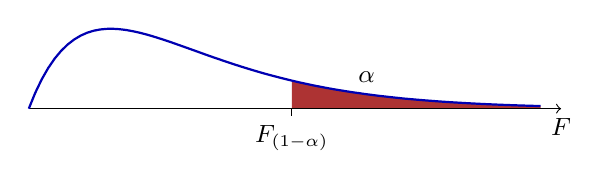
\begin{tikzpicture}[xscale=1.3,yscale=2.2]
    \fill[red!60!black,opacity=0.8,domain=2.57:5,samples=40] (2.57,0) -- plot (\x,{0.95*\x*exp(-1.25*\x)*1.65}) -- (5,0) -- cycle;
    \draw[->] (0,0) -- (5.2,0) node[below]{\small $F$};
    \draw[thick,blue!70!black,domain=0:5,samples=80] plot (\x,{0.95*\x*exp(-1.25*\x)*1.65});
    \draw (2.57,0) -- (2.57,-0.04) node[below]{\small $F_{(1-\alpha)}$};
    \node at (3.3,0.18) {\small $\alpha$};
\end{tikzpicture}
\\[2pt] \textit{\small Only the right tail is used.}
\end{center}

\begin{definition}[Concluding the ANOVA Test]
    If p-value $<\alpha$, or $F^*>F_{(1-\alpha),(p,\,n-p-1)}$, reject $H_0$ and conclude a
    statistically significant linear relationship exists for \textbf{at least one} predictor.
\end{definition}

\begin{example}[House Pricing, Manually]
    $H_0:\beta_1=\beta_2=0$ vs.\ $H_A$: at least one $\beta_j\neq0$.
    \begin{enumerate}
        \item \textbf{Degrees of freedom}: $n=100$, $p=2$; $df_{RSS}=100-2-1=97$, $df_{SST}=99$, $df_{SS_{reg}}=2$.
        \item \textbf{Sums of squares} (R for the middle steps):
        \[SST=(n-1)s_y^2=99(81.99404)=8117.41,\qquad RSS=(n-p-1)s^2=982.114,\]
        \[SS_{reg}=SST-RSS=7135.296\]
\begin{verbatim}
var(sellPrice)                              # 81.99404
sum((model$fitted.values - sellPrice)^2)    # 982.114
\end{verbatim}
        \item \textbf{Mean squares}: $MSR=\frac{982.114}{97}=10.12489$, $MS_{reg}=\frac{7135.296}{2}=3567.648$.
        \item \textbf{Test statistic}: $F^*=\frac{3567.648}{10.12489}=\hlt{352.36}$.
        \item \textbf{Conclusion} (p-value or critical value):
\begin{verbatim}
pf(352.36, 2, 97, lower.tail = FALSE)   # F*, df1, df2, right tail only
# 3.260824e-45
qf(0.95, 2, 97)                         # 3.090187
\end{verbatim}
        \dbb{Reject $H_0$}: a significant linear relationship exists for at least one predictor.
    \end{enumerate}
    \aside{Also $R^2=SS_{reg}/SST=7135.296/8117.41=0.879$, matching the summary.}
    In R, the overall test is the last line of \texttt{summary()}:
    \texttt{F-statistic: 352.4 on 2 and 97 DF, p-value: < 2.2e-16} ($F^*$, $df_1$, $df_2$).
\end{example}

\subsection{Partial $F$ Test}

\begin{remark}[Testing a Subset of Predictors]
    Suppose a model with $X_1,X_2,X_3$: the overall ANOVA test says at least one predictor is
    related to $Y$, and the $t$-tests say only $X_3$ is significant. Is the simple model with
    only $X_3$ as good as the 3-predictor model?
    \begin{itemize}
        \item Can we remove the two insignificant predictors \textbf{at the same time}? Since each
        predictor is conditionally related to $Y$, the $t$-test only says you can remove them
        one at a time (not together).
        \item A \textbf{partial $F$ test} tells us whether both can be removed simultaneously.
        If the simple model is as good, $SS_{reg}$ and $RSS$ should be similar between the two
        models; if the reduced model's RSS is too much bigger, it explains less of the variation
        in $Y$ and we can't remove all the insignificant predictors at once.
    \end{itemize}
\end{remark}

\begin{definition}[Full and Reduced Models]
    A partial $F$ test compares 2 models fit to the same data/response (so $SST$ is the same):
    \begin{itemize}
        \item \textbf{Complete/full} model (the bigger one) with $p$ predictors;
        \item \textbf{Reduced} model (the smaller one) with $p-k$ predictors ($k$ removed).
    \end{itemize}
    A model with more predictors (even non-significant ones) has smaller RSS:
    \[RSS_{reduced}\geq RSS_{full}\iff SS_{reg,reduced}\leq SS_{reg,full}\]
    so we adjust for the additional predictors by standardizing with each model's df.
\end{definition}

\begin{definition}[Partial $F$ Test]
    Write $\boldsymbol\beta=(\beta_0,\boldsymbol\beta_1,\boldsymbol\beta_2)'$, where
    $\boldsymbol\beta_1$ holds the $p-k$ coefficients to \textbf{keep} and $\boldsymbol\beta_2$
    the $k$ coefficients we \textbf{consider dropping}. Test
    \[H_0:\boldsymbol\beta_2=\mathbf{0}\ \ (\beta_{p-k+1}=\cdots=\beta_p=0)\quad\text{vs.}\quad H_A:\boldsymbol\beta_2\neq\mathbf{0}\ \ (\text{at least one}\neq0)\]
    Quantify the difference in RSS:
    \[RSS_{drop}=RSS_{reduced}-RSS_{full}=SS_{reg,full}-SS_{reg,reduced}\]
    \begin{itemize}
        \item Full model better: it explains more of the variation in $Y$, $RSS_{full}$ is much
        smaller than $RSS_{reduced}$ $\Rightarrow$ \textbf{bigger} $RSS_{drop}$.
        \item Similar models: a similar amount of variation is explained, the RSS's are similar
        $\Rightarrow$ \textbf{smaller} $RSS_{drop}$.
    \end{itemize}
    Like the ANOVA test, compare the mean SS difference to the model with the smallest
    mean squares residual (the full model):
    \[\boxed{F^*=\frac{RSS_{drop}/k}{RSS_{full}/(n-p-1)}\sim F(k,\,n-p-1)\text{ under }H_0}\]
    \aside{If the reduced model is $y\sim1$, this is exactly the ANOVA overall test statistic.}
\end{definition}

\heading{Concluding the Partial $F$ Test}
$H_0$ says the larger (full) model is not better than the smaller (reduced) model
($MSR_{drop}$ small relative to $MSR_{full}$).
\begin{itemize}
    \item If $F^*<F_{(1-\alpha),(k,\,n-p-1)}$: \textbf{fail to reject} $H_0$. The additional
    $SS_{reg}$ from the $k$ predictors isn't enough to keep them \aside{(the outcome we want if
    aiming for simpler models)}. Conclude no significant linear relationship between $Y$ and
    \underline{any} of the $k$ predictors.
    \item If $F^*>F_{(1-\alpha),(k,\,n-p-1)}$ or p-value $<\alpha$: \textbf{reject} $H_0$. The
    additional $SS_{reg}$ explains a lot of variation, so keep these predictors. Conclude a
    significant linear relationship exists between $Y$ and \underline{\textbf{at least one}} of
    the $k$ predictors we tried dropping.
\end{itemize}

\begin{example}[Iris Dataset]
    Edgar Anderson's iris data (built into R as \texttt{iris}): 150 flowers, 50 from each of
    3 species (setosa, versicolor, virginica), with sepal/petal length and width in cm. Model
    petal length by petal width and species:
    \[\text{Length}=\beta_0+\beta_1\text{Width}+\beta_2I(\text{Species}=\text{versicolor})+\beta_3I(\text{Species}=\text{virginica})+\epsilon\]
\begin{verbatim}
model2 <- lm(Petal.Length ~ Petal.Width + Species, data = iris)

                  Estimate Std. Error t value Pr(>|t|)
(Intercept)        1.21140    0.06524  18.568  < 2e-16 ***
Petal.Width        1.01871    0.15224   6.691 4.41e-10 ***
Speciesversicolor  1.69779    0.18095   9.383  < 2e-16 ***
Speciesvirginica   2.27669    0.28132   8.093 2.08e-13 ***
Residual standard error: 0.3777 on 146 degrees of freedom
Multiple R-squared: 0.9551, Adjusted R-squared: 0.9542
F-statistic: 1036 on 3 and 146 DF, p-value: < 2.2e-16
\end{verbatim}
    \textbf{Can we omit species?} We can't use the $t$-test since multiple $\beta_j$'s
    correspond to Species; we want to test $\beta_2=\beta_3=0$ simultaneously ($\beta_1$ for
    petal width stays). Use the partial $F$ test.
\end{example}

\begin{example}[Iris: Partial $F$ Test by Hand]
    $H_0:\beta_2=\beta_3=0$ vs.\ $H_A$: at least one of $\beta_2,\beta_3\neq0$.
    \begin{enumerate}
        \item \textbf{Models and RSS}: full \texttt{length \textasciitilde{} width + species},
        reduced \texttt{length \textasciitilde{} width}.
\begin{verbatim}
y <- iris$Petal.Length
sum((model2$fitted.values - y)^2)           # 20.83344 (full)
sum((model2_reduced$fitted.values - y)^2)   # 33.84475 (reduced)
\end{verbatim}
        \item $RSS_{drop}=RSS_{reduced}-RSS_{full}=33.84475-20.83344=13.01131$.
        \aside{Always positive ($RSS_{full}$ is always smaller than $RSS_{reduced}$); if
        negative, check the order of subtraction.} We dropped 2 $\beta$'s, so $k=2$.
        \item \textbf{Test statistic}:
        \[F^*=\frac{RSS_{drop}/k}{RSS_{full}/(n-p-1)}=\frac{13.01131/2}{20.83344/(150-3-1)}=45.5914\]
        \item \textbf{Conclusion}: \texttt{pf(45.5914, 2, 146, lower.tail = FALSE)} $=4.137\times10^{-16}$
        $\Rightarrow$ \dbb{reject $H_0$}: we cannot remove species from the full model.
    \end{enumerate}
\end{example}

\begin{example}[Iris: Partial $F$ Test Using R]
    Fit the model without species as the reduced model, then call \texttt{anova(reduced, full)}:
\begin{verbatim}
model2_reduced <- lm(Petal.Length ~ Petal.Width, data = iris)
anova(model2_reduced, model2)   # anova(reduced, full)

Model 1: Petal.Length ~ Petal.Width
Model 2: Petal.Length ~ Petal.Width + Species
  Res.Df    RSS Df Sum of Sq      F    Pr(>F)
1    148 33.845
2    146 20.833  2    13.011 45.591 4.137e-16 ***
\end{verbatim}
    \aside{Even by hand, it helps to organize calculations in a table like this output.}
\end{example}

\subsection{Relationships Between the Tests}

\heading{Considerations for Using These Tests}
\begin{itemize}
    \item General order (a guideline, not the law): \textbf{ANOVA overall test $\to$ $t$-tests
    on individual coefficients $\to$ partial $F$ test}. The $t$-tests help inform which
    predictors you might consider dropping.
    \item Always check assumptions before any hypothesis test; for $F$ tests, verify them in
    \textbf{both} the full and reduced models.
    \item Cautions for the partial $F$ test:
    \begin{itemize}
        \item cannot compare models from different datasets;
        \item cannot compare models unless one is \textbf{nested} in (a subset of) the other ---
        e.g.\ with model 1: $X_1,X_2,X_3$, model 2: $X_2,X_4$, model 3: $X_2,X_3$, only models 1
        and 3 can be compared.
    \end{itemize}
    \item To remove one categorical predictor with more than 2 categories, we \textbf{must} use
    the partial $F$ test (testing multiple $\beta_j$'s $=0$ simultaneously).
\end{itemize}

\begin{example}[ANOVA Overall Test as a Partial $F$ Test]
    The reduced model is the intercept-only model; same $F^*$ as the \texttt{lm()} summary and
    the manual calculation:
\begin{verbatim}
anova(lm(sellPrice ~ 1), model)

Model 1: sellPrice ~ 1
Model 2: sellPrice ~ numBedrooms + numBathrooms
  Res.Df    RSS Df Sum of Sq      F    Pr(>F)
1     99 8117.4
2     97  982.1  2    7135.3 352.36 < 2.2e-16 ***
\end{verbatim}
\end{example}

\begin{remark}[$F$-Test vs.\ $t$-Test]
    \begin{itemize}
        \item $t$-test: $H_0:\beta_j=0$ for a single parameter. $F$-test: $H_0:\beta_1=\beta_2=\cdots=0$,
        the \textbf{joint} significance of multiple predictors.
        \item Can we run the $t$-test $k$ times instead? \textbf{No!} The $F$-test works under
        multicollinearity (high correlation among predictors); the $t$-test does not.
        \item For \textbf{SLR}, the partial $F$-test, ANOVA overall test and $t$-test of
        $H_0:\beta_1=0$ are all equivalent.
        \item Removing only \textbf{one} $\beta$ in MLR, the partial $F$-test is equivalent to the $t$-test.
    \end{itemize}
    In both equivalent cases, $\boxed{F^*=(t^*)^2}$ with the same p-value, since
    \[t=\frac{N(0,1)}{\sqrt{\chi^2_{df}/df}}\quad\Rightarrow\quad t^2=\frac{\chi^2_1/1}{\chi^2_{df}/df}\sim F(1,df)\]
\end{remark}

\begin{example}[$F^*=(t^*)^2$ in the House Pricing Data]
    \textbf{Removing one predictor} from \texttt{sellPrice \textasciitilde{} numBedrooms + numBathrooms}:
\begin{verbatim}
anova(lm(sellPrice ~ numBathrooms), model)
#   Res.Df    RSS Df Sum of Sq      F Pr(>F)
# 1     98 993.08
# 2     97 982.11  1    10.969 1.0834 0.3005
anova(lm(sellPrice ~ numBedrooms), model)
# 1     98 993.46
# 2     97 982.11  1    11.351 1.1211 0.2923
\end{verbatim}
    matching the $t$-tests: $1.041^2=1.0837$ (p $=0.30053$) for \texttt{numBedrooms} and
    $1.059^2=1.1215$ (p $=0.29232$) for \texttt{numBathrooms} \aside{(up to rounding of $t^*$)}.
    \\ \textbf{SLR}: \texttt{anova(lm(sellPrice\textasciitilde1), lm(sellPrice\textasciitilde numBedrooms))}
    gives $F^*=702.74$ on 1 and 98 df, the summary's $F$-statistic is 702.7, and $26.509^2=702.73$.
\end{example}

\begin{remark}[Module Takeaways]
    \begin{itemize}
        \item What do the components of the sum of squares decomposition measure, and how are
        they computed?
        \item What is the difference between the hypotheses for the ANOVA test and the partial $F$ test?
        \item How is the decomposition used differently in each, how do we conduct each test,
        and what are their conclusions?
    \end{itemize}
\end{remark}
